\section{Results}\label{sec:result}

Given a SPN primitive and $A$, the maximum S-boxes to be considered, we first generate graph $G$ according to our method in Section \ref{algo:gen_G}. Applying our method in Section \ref{algo:find_ite_c_G}, we find the best iterative characteristic in $G$. Applying our method in Section \ref{algo:find_ite_h_G}, we find the best iterative hull. Comparing the two results, we show the strength of the clustering effect through a bar chart. Applying our method in Section \ref{algo:msg}, we estimate the EDPs and ELPs for these ciphers. 

\subsection{Results on Iterative Characteristics and Hulls}

We apply our algorithms in Section \ref{sec:find_ite_c} and \ref{sec:find_ite_h} to SPN ciphers including RECTANGLE, PRESENT, GIFT and so on. Note that a iterative distinguisher is used to build a longer distinguisher, thus we keep the iterative distinguishers we consider with small number of rounds. In our experiments, we set the biggest number of rounds to be 10. We show results on differential cryptanalysis in Figure \ref{fig:bar_ddt} and results linear cryptanalysis in Figure \ref{fig:bar_lat2}. The blue bars are obtained applying our method in Section \ref{sec:find_ite_c} searching the best elementary iterative characteristics with no more than 10 rounds. The orange bars are obtained by computing the minimum value applying our method in Section \ref{sec:find_ite_h} given $r=1:10$. Comparing the two figures, it is shown that linear characteristics are more likely to cluster than diffrential ones. 

\begin{figure}\label{fig:bar_ddt}
    \centering
    \caption{Results on iterative differential characteristics for some SPN block ciphers including RECTANGLE, PRESENT, GIFT64, PUFFIN and TRIFLE. The y-axis is the negative logarithm of differential probabilities. The blue bars are the weight growth of the best iterative characteristics. The orange bars are the weight growth of the best iterative hulls.}
	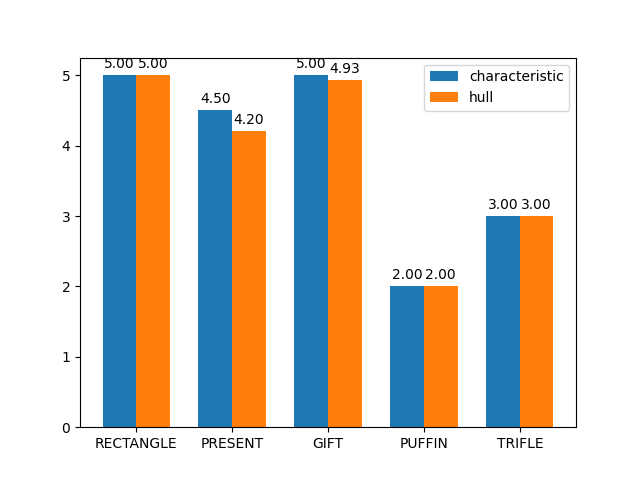
\includegraphics[width=0.8\textwidth]{fig/bar_ddt.png}
\end{figure}

\begin{figure}\label{fig:bar_lat2}
    \centering
    \caption{Results on iterative linear characteristics for some SPN block ciphers including RECTANGLE, PRESENT, GIFT64, PUFFIN, EPCBC and TRIFLE. The y-axis is the negative logarithm of linear correlation squares. The blue bars are the weight growth of the best iterative characteristics. The orange bars are the weight growth of the best iterative hulls.}
	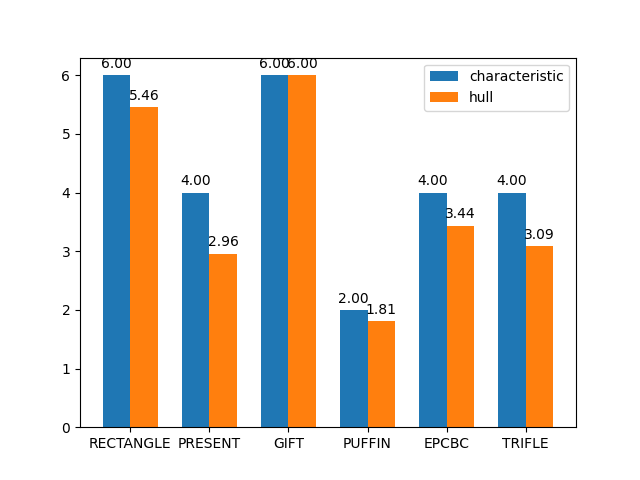
\includegraphics[width=0.8\textwidth]{fig/bar_lat2.png}
\end{figure}

In the following, we list the experimental settings and results for each of the ciphers. 



\subsubsection{PRESENT \cite{bogdanov2007present}} We set $A=3$ in the differential case and $A=1$ in the linear case. The best differential characteristic is exactly the one given in \cite{wang2008differential}. In \cite{ohkuma2009weak}, the author

\subsubsection{RECTANGLE \cite{zhang2015rectangle}} All operations of RECTANGLE has the rotational symmetry and thus we set the equivalance relation to be $=_R$. We set $A=3$ in both cases of differential and linear cryptanalysis. In the case of linear cryptanalysis, we can find better distinguishers considering the clustering effect. 

\subsubsection{GIFT \cite{banik2017gift}} We set $A=3$ in both differential and linear cases. GIFT has a very weak clustering effect in both case of differential and linear cryptanalysis. 

\subsubsection{PUFFIN \cite{cheng2008puffin}} We set $A=1$ in both differential and linear cases.  

\subsubsection{EPCBC \cite{yap2011epcbc}} We set $A=1$ in the linear case. We can't find any iterative differential characteristic though $A$ is set up to 3. 

\subsubsection{TRIFLE-BC \cite{Datta2019trifle}} We set $A=1$ in both diffrential and linear cases. 

%\begin{figure}\label{fig:plot_ite}
%    \centering
%    \caption{Results on some SPN block ciphers, which are RECTANGLE, PRESENT, GIFT64, PUFFIN, EPCBC and TRIFLE from top to bottom resp. For each subfigure, the x-axis is the number of rounds. For a subfigure in the left column, the y-axis is the weight of differential probability, while for a subfigure in the right column, the y-axis is the weight of correlation square. The red spot denotes the best single iterative characteristic with fewest rounds obtained by Algo. \ref{algo:find_ite_c_G}. The yellow (green, blue) line denotes the best iterative hull with $A=$1 (2, 3).} 
%	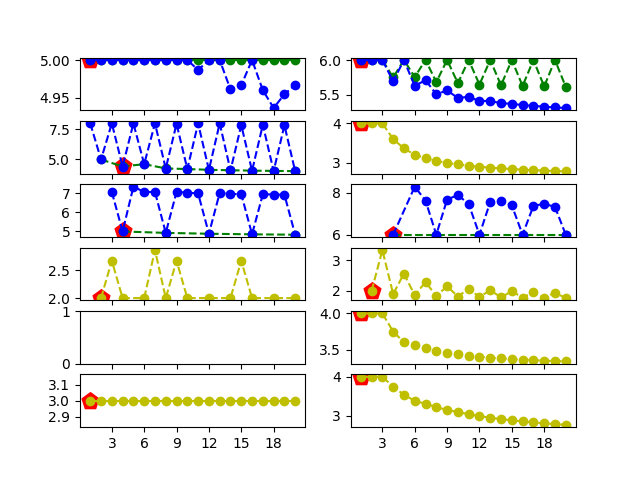
\includegraphics[width=1\textwidth]{fig/iterative.png}
%\end{figure}

\subsection{Results on Estimating EDPs and ELPs}

We apply our algorithm in Section \ref{sec:method-edp-elp} to some SPN primitives. The results are given in Table \ref{tab:EDP} and Table \ref{tab:ELP}. 

\begin{table}
	\caption{Results on estimating EDPs. $r$ is the number of rounds. $A$ is the maximum number of S-boxes which the differences we consider can have. $(k,log_2wlb)$ determines the scope of extended differential characteristics we consider. $\Prob$ is the probability of the best differential characteristic we find. $\EDP$ is obtained by our method in Section \ref{sec:method-edp-elp}. $T_g$ and $T_s$ are the running times generating and searching the multistage graph}\label{tab:EDP}
	\centering
	\begin{tabular}{|c|c|c|c|c|c|c|}
		\hline
		cipher & $r$ & $A$ & $(k,-\log_2wlb)$ & $-\log_2\Prob$ & $-\log_2\EDP$ & $T_g+T_s$ \\
		\hline
		PRESENT & 16 & 2 & (3,10) & 70 & 61.84 & 26s+165s\\
		\hline
		GIFT-64 & 13 & 2 & (3,13) & 62 & 60.42 & 24s+76s\\
		\hline 
		RECTANGLE & 14 & 2 & (6,25) & 61 & 60.65 & 4s+133.1h \\
		\hline
		KNOT-perm-256 & 52 & 2 & (3,12) & 274 & 251.831 & 0s+10s\\
		\hline
	\end{tabular}
\end{table}

\begin{table}
	\caption{Results on estimating ELPs. $r$ is the number of rounds. $A$ is the maximum number of S-boxes which the masks we consider can have. $(k,log_2wlb)$ determines the scope of extended linear characteristics we consider. $\Cor$ is the correlation of the best linear characteristic we find. $\ELP$ is obtained by our method in Section \ref{sec:method-edp-elp}. $T_g$ and $T_s$ are the running times generating and searching the multistage graph}\label{tab:ELP}
	\centering
	\begin{tabular}{|c|c|c|c|c|c|c|}
		\hline
		cipher & $r$ & $A$ & $(k,-\log_2wlb)$ & $-2\log_2\Cor$ & $-\log_2\ELP$ & $T_g+T_s$ \\
		\hline
		PRESENT & 24 & 1 & (3,8) & 92 & 63.61 & 0s+14s\\
		\hline
		GIFT-64 & 13 & 2 & (3,10) & 64 & 64 & 1s+1s\\
		\hline 
		RECTANGLE & 14 & 3 & (3,14) & 68 & 62.31 & 17s+1.5h \\
		\hline
		KNOT-perm-256 & 56 & 3 & (2,6) & 161 & 125.262 & 27s+6.0h\\
		\hline
	\end{tabular}
\end{table}

\subsubsection{Comparison with the results in \cite{EPRINT:HalVej18}}

We find that our results are very close to the results obtained in \cite{EPRINT:HalVej18}, which implies that the assumption that the best differential or linear distinguisher for an S-bP symmetric-key primitive is dominated by iterative characteristics is reasonable. 

\subsection{Results on differential and linear attacks against KNOT-AEAD and KNOT-Hash}

KNOT is a family of lightweight authenticated encryption algorithms and hash functions \cite{zhang2019knot}. The modes of operation of KNOT for AE and hash are shown in Figure \ref{fig:mode_aead},\ref{fig:mode_hash}. The modes are similar to the ones used in Ketje \cite{bertoni2014ketje} and ASCON \cite{dobraunig2016ascon}. The inner permutations are inheritors of RECTANGLE, which are bit-sliced lightweight. The round transformation has 3 steps: 4-bit S-boxes, row rotations and a constant addition. 

\begin{figure}
	\centering
	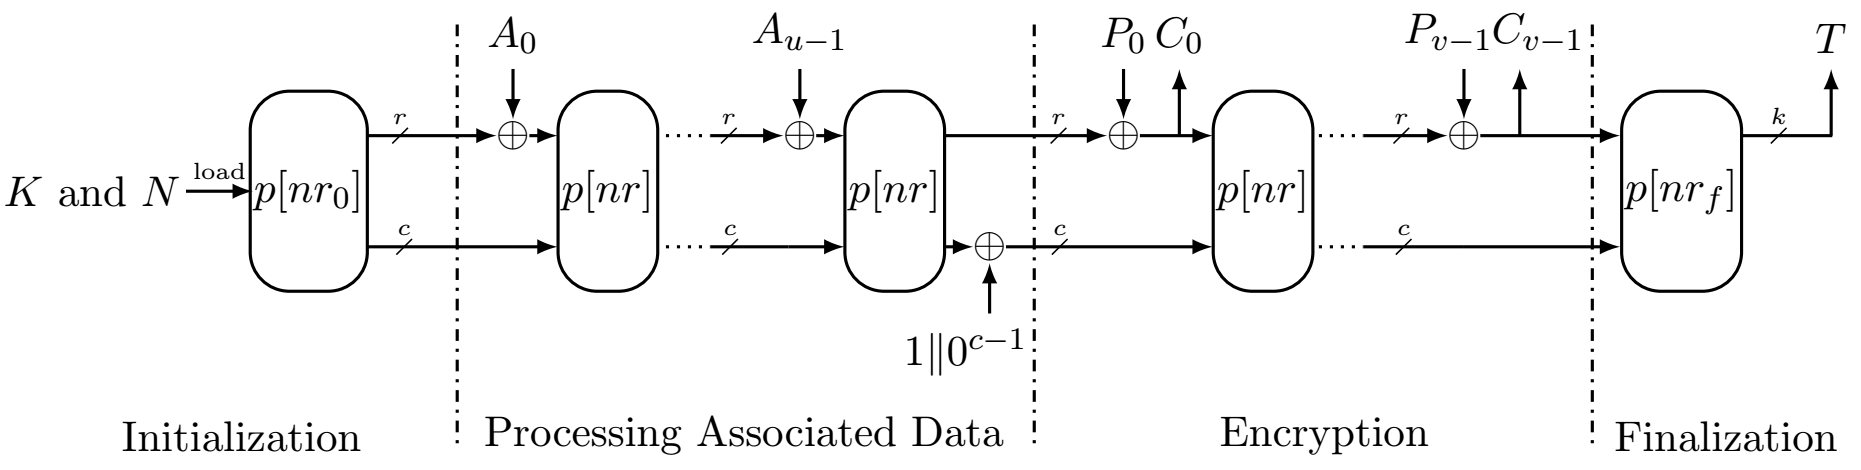
\includegraphics[width=1\textwidth]{fig/mode_aead.PNG}
	\caption{The operation mode of KNOT AEAD} \label{fig:mode_aead}
\end{figure}

\begin{figure}
	\centering
	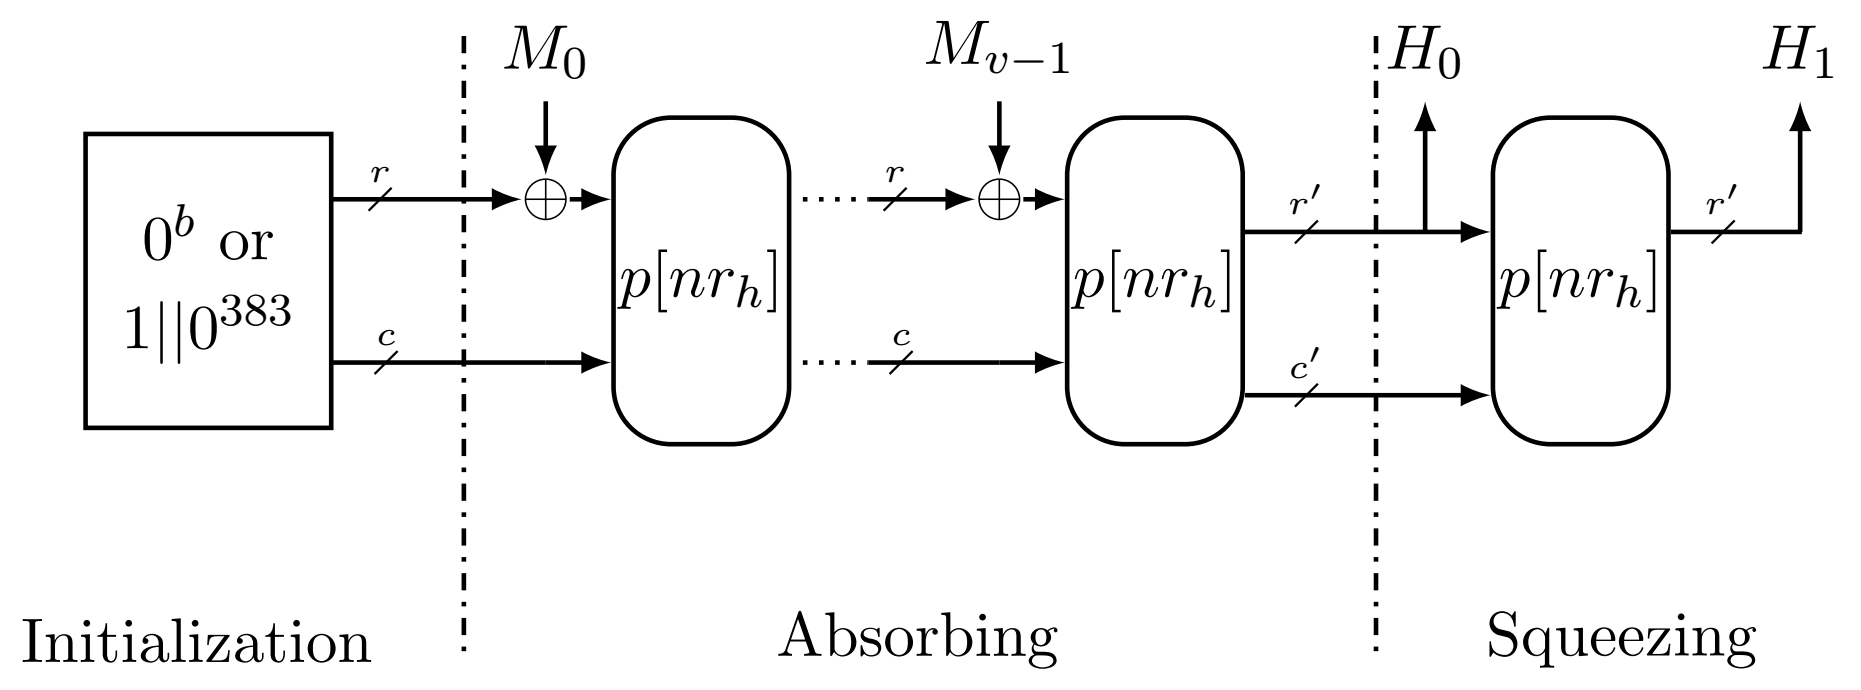
\includegraphics[width=0.7\textwidth]{fig/mode_hash.PNG}
	\caption{The operation mode of KNOT Hash} \label{fig:mode_hash}
\end{figure}

In the original specification document of KNOT, The largest differential probability and linear correlation is given. However firstly, the differential and linear distinguishers with no restrictions can not be directly uesd to attack the MonkeyDuplex construction. Secondly, the clustering effect is not taken into consideration. Thirdly, because only the rate part and the tag part is visible, differences can be truncated in the capacity part and in the non-tag part. 

In the following, we propose differential and linear attacks targeting different phases, each demanding specific restrictions on the distinguishers. The attacks proposed are general for cryptographic schemes based on MonkeyDuplex construction. For each attack, we give the largest differential probability or linear correlation square of the longest distinguisher as in Table \ref{tab:knot}. 

\begin{itemize}
	\item \textbf{Diff-Init-D} This is a chosen-nonce differential distinguishing attack targeting the initialization phase of KNOT-AEAD. The input difference has the nonce part and key part $\Delta SI=(\Delta SI_N,\Delta SI_K)$. The output difference has the rate part and capacity part $\Delta SO=(\Delta SO_R,\Delta SO_C)$. We restrict that $\Delta SI_K=0$. And $\Delta SO_C$ is truncated. 
	\item \textbf{Linear-Init-KR} This is a known-nonce and known-plaintext linear key recovery attack targeting the initialization phase of KNOT-AEAD. The input mask $\Gamma SI=(\Gamma SI_N,\Gamma SI_K)$ and the output mask $\Gamma SO=(\Gamma SO_R,\Gamma SO_C)$. We restrict that $\Gamma SO_C=0$. Note that if for the best linear distinguisher $\Gamma SI_K\neq 0$, then the attack degrades to a distinguishing one, of which the probability is negligible. 
	\item \textbf{Linear-Enc-D} This is a known-plaintext linear distinguishing attack targeting the encryption phase of KNOT-AEAD. The input mask $\Gamma SI=(\Gamma SI_R,\Gamma SI_C)$ and the output mask $\Gamma SO=(\Gamma SO_R,\Gamma SO_C)$. We restrict that $\Gamma SI_C=0$ and $\Gamma SO_C=0$. 
	\item \textbf{Diff-Enc-F} This is a differential forgery attack targeting the encryption phase of KNOT-AEAD. The input difference $\Delta SI=(\Delta SI_R,\Delta SI_C)$ and the output difference $\Delta SO=(\Delta SO_R,\Delta SO_C)$. We restrict that $\Delta SI_C=0$ and $\Delta SO_C=0$. 
	\item \textbf{Diff-Final-F} This is a differential forgery attack targeting the finalization phase of KNOT-AEAD. The input difference $\Delta SI=(\Delta SI_R,\Delta SI_C)$ and the output difference $\Delta SO=(\Delta SO_T,\Delta SO_{nT})$. We restrictions that $\Delta SI_C=0$. And $\Delta SO_{nT}$ is truncated. 
	\item \textbf{Diff-Col-ABS} This is a differential collsion attack targeting the absorb phase of KNOT-Hash. The input difference $\Delta SI=(\Delta SI_R,\Delta SI_C)$ and the output difference $\Delta SO=(\Delta SO_R,\Delta SO_C)$. We restrictions that $\Delta SI_C=0$ and $\Delta SO_C=0$. 
	\item \textbf{Diff-Col-SQZ} his is a differential collsion attack targeting the squeezing phase of KNOT-Hash. The input difference $\Delta SI=(\Delta SI_R,\Delta SI_C)$ and the output difference $\Delta SO=(\Delta SO_{R'},\Delta SO_{C'})$. We restrictions that $\Delta SI_C=0$ and $\Delta SI_{R'}=0$. And $\Delta SI_{C'}$ is truncated. 
\end{itemize}

\begin{table}
	\caption{Results for the primary version of KNOT}\label{tab:knot}
	\centering
	\begin{tabular}{|c|c|c|c|c|c|c|c|}
		\hline
		Attack Model & $r$ & $A$ & $(k,-\log_2wlb)$ & $-\log_2$(EDP or ELP)\\
		\hline
		Diff-Init-D & 14 & 2 & (5,20) & 62.2 \\
		Linear-Init-KR & 13 & 3 & (3,8) & 30.7*2=61.4 \\
		Linear-Enc-D & 12 & 3 & (3,10) & 30.2*2=60.4 \\
		Diff-Enc-F & 12 & 2 & (5,20) & 62.4 \\
		Diff-Final-F & 13 & 2 & (5,20) & 61.4 \\
		Diff-Col-ABS & 12 & 2 & (5,20) & 62.7 \\
		Diff-Col-SQZ & 13 & 2 & (5,20) & 61.4 \\
		\hline
	\end{tabular}
\end{table}

\subsubsection{Comparison with the method of enumerating characteristics}

To verify our results, fixing the input and output differences (masks) as those obtained using our method, we use the MILP method to evaluete the EDPs (ELPs) by enumerating characteristics with their differential probabilities (linear amplitudes) larger than a bound. We respectively check on a 10-round differential and a 10-round linear approximation.

For the 10-round differential $\alpha[32]=1,\alpha[49]=1\rightarrow \beta[39]=1,\beta[63]=1$, the differential probability obtained by our method is $2^{-53.7}$ while that obtained by the MILP method is $2^{53.5}$. 

For the 10-round linear approximation $\alpha[0]=1,\alpha[25]=1\rightarrow \beta[24]=1,\beta[41]=1$, the linear correlation amplitude obtained by our method is $2^{-26.4}$ while that obtained by the MILP method is $2^{-25.5}$. We list the number of characteristics considered in both methods in Table \ref{tab:num-linear}. Our method underestimates the correlation amplitude for some characteristics with correlation amplitudes no smaller than $2^{34}$ are missing. But it holds that the distinguisher is dominated by iterative characteristics. 

\begin{table}
	\caption{Results on the number of characteristics of the 10-round linear approximation grouped by the correlation amplitude}\label{tab:num-linear}
	\centering
	\begin{tabular}{|c|c|c|c|c|c|c|c|c|c|c|c|c|c|c|}
		\hline
		$\log_2|\Cor|$ & 30 & 31 & 32 & 33 & 34 & 35 & 36 & 37 & 38 & 39 & 40 & 41 & 42 & 43\\
		\hline
		MILP & 8 & 0 & 72 & 4 & 264 & 72 & 648 & 364 & 1260 & 1092 & - & - & - & -\\
		\hline
		ours & 8 & 0 & 72 & 4 & 248 & 48 & 392 & 132 & 252 & 148 & 60 & 36 & 12 & 4\\
		\hline
	\end{tabular}
\end{table}

\subsection{Visualization of the Iterative Structure}

Taking the differential iterative structure of RECTANGLE as an example, we present all its edges in Table \ref{tab:dis-rect}. We show its graph presentation in Figure \ref{fig:dis-rect}. The red parts are the strong components which containing all iterative characteristics. The blue parts contain one-way paths linking different strong components. 

We hope the visualization of the iterative structure of a symmetric-key primitive may reveal some insights on cipher designing. 

\begin{figure}\label{fig:dis-rect}
    \centering
    \caption{Visualization of the differential iterative structure of RECTANGLE when $A=2$. The red parts are the strong components. The blue parts are one-way paths linking different strong components. }
	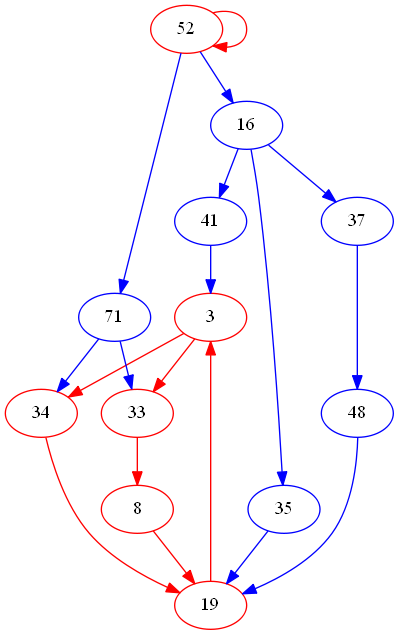
\includegraphics[width=0.3\textwidth]{fig/test_circuits.png}
\end{figure}

\begin{table}
	\caption{The differential iterative structure of RECTANGLE when $A=2$}\label{tab:dis-rect}
	\centering
	\begin{tabular}{|c|c|c|c|c|c|}
		\hline
		head No. & head difference & tail No. & tail difference & $d$ & $\Prob$ \\
		\hline
		3 & 8c00000000000000 & 33 & 3000c00000000000 & 0 & $2^{-5}$ \\
        3 & 8c00000000000000 & 34 & 3000800000000000 & 0 & $2^{-5}$ \\
        8 & 800000000000a000 & 19 & 500000000000000a & 0 & $2^{-6}$ \\
        16 & 6000000000000008 & 35 & 3000400000000000 & 15 & $2^{-5}$ \\
        16 & 6000000000000008 & 37 & 3000000000000000 & 15 & $2^{-5}$ \\
        16 & 6000000000000008 & 41 & 2300000000000000 & 14 & $2^{-5}$ \\
        19 & 500000000000000a & 3 & 8c00000000000000 & 2 & $2^{-5}$ \\
        33 & 3000c00000000000 & 8 & 800000000000a000 & 7 & $2^{-5}$ \\
        34 & 3000800000000000 & 19 & 500000000000000a & 4 & $2^{-6}$ \\
        35 & 3000400000000000 & 19 & 500000000000000a & 4 & $2^{-5}$ \\
        37 & 3000000000000000 & 48 & 2000800000000000 & 15 & $2^{-3}$ \\
        41 & 2300000000000000 & 3 & 8c00000000000000 & 3 & $2^{-6}$ \\
        48 & 2000800000000000 & 19 & 500000000000000a & 4 & $2^{-6}$ \\
        52 & 2000060000000000 & 16 & 6000000000000008 & 4 & $2^{-5}$ \\
        52 & 2000060000000000 & 52 & 2000060000000000 & 15 & $2^{-5}$ \\
        52 & 2000060000000000 & 71 & 2000000000000008 & 4 & $2^{-5}$ \\
        71 & 2000000000000008 & 33 & 3000c00000000000 & 15 & $2^{-6}$ \\
        71 & 2000000000000008 & 34 & 3000800000000000 & 15 & $2^{-6}$ \\
		\hline
	\end{tabular}
\end{table}